\documentclass[12pt, a4, twoside]{article}
\usepackage[utf8]{inputenc}
\usepackage{graphicx}
\usepackage{algorithm}
\usepackage{algpseudocode}
\usepackage{amsmath}
\usepackage{amsfonts}
\usepackage{hyperref}
\usepackage{mathtools}
\DeclarePairedDelimiter\ceil{\lceil}{\rceil}
\DeclarePairedDelimiter\floor{\lfloor}{\rfloor}

\hypersetup{
    colorlinks=true,
    linkcolor=blue,
    filecolor=magenta,
    urlcolor=cyan,
}

\usepackage[backend=bibtex]{biblatex}
\addbibresource{fast-direct-solvers.bib}

\title{Fast Direct Solvers for the Solution of Integral Equations}
\author{Srinath Kailasa \thanks{srinath.kailasa.18@ucl.ac.uk} \\ \small University College London}

\date{\today}

\begin{document}

\maketitle

\section*{Abstract}
So called `fast direct solvers' offer an $O(N)$ alternative to iterative methods ($O(n_{iter} \cdot n)$) for the solution of integral equations, and therefore are a rapidly developing field of research. In this document, I summarise the recent research in this direction in the context of computing the solution of acoustic and electromagnetic scattering problems which have been formulated as integral equations. \footnote{These notes were written up during my visit to the Flatiron Institute in New York City in the Summer of 2022. A wonderful experience for which I am extremely grateful. The visit gave me both the impetus and the time to study some truly interesting and beautiful concepts.}.

\newpage

\tableofcontents

\section{A Hierarchical Matrix Zoo}

The matrices that we're concerned with are in some sense `data-sparse', in that the off-diagonal elements are in some way `small', and compressible without a great deal of information loss.

Figures (\ref{fig:hierarchical_matrices}) and (\ref{fig:hierarchical_matrices_2}) from Ambikasaran \cite{Ambikasaran2013}, summarizes the main types of matrices that arise when discretising integral equations and their relationship to each other. In the context of hierarchical matrices and fast direct solvers, \textit{\textbf{Admissibility}} refers to whether neighbour boxes are considered low-rank (weak), or whether only non-adjacent children of the parent box's neighbours are considered low-rank (strong). \textit{\textbf{Nested Basis}}, are related to the ability to form the basis for a given box using that of its children.


\begin{figure}[!h]
    \centering
    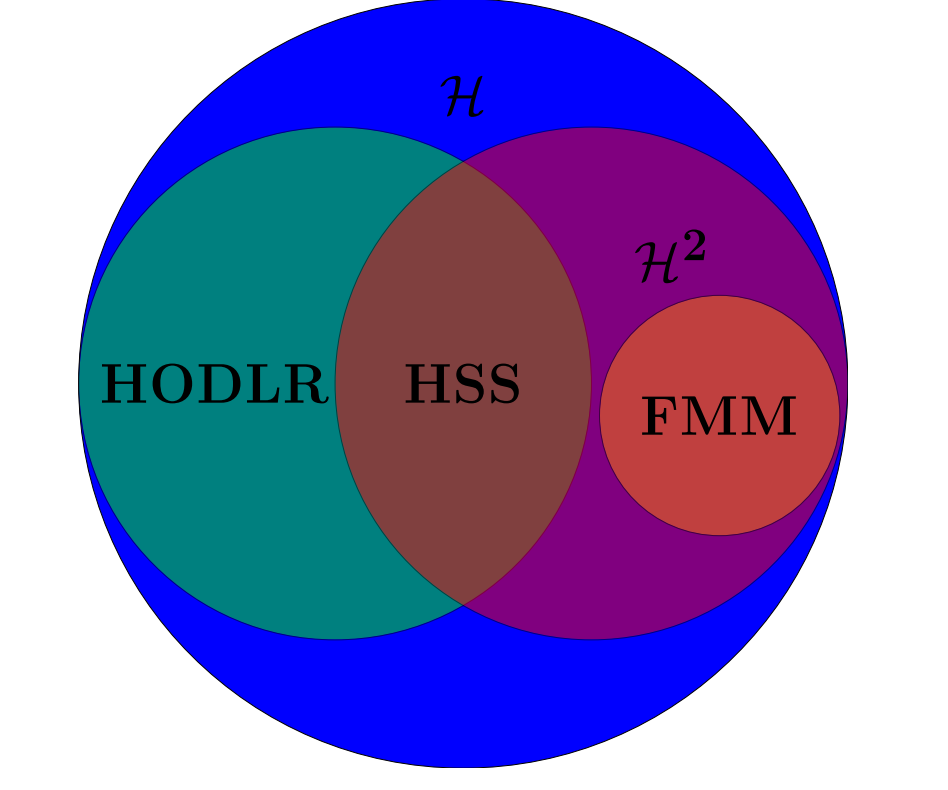
\includegraphics[width=0.6\textwidth]{euler.png}
    \caption{Taxonomy of hierarchical matrices.}
    \label{fig:hierarchical_matrices}
\end{figure}


\begin{figure}[!h]
    \centering
    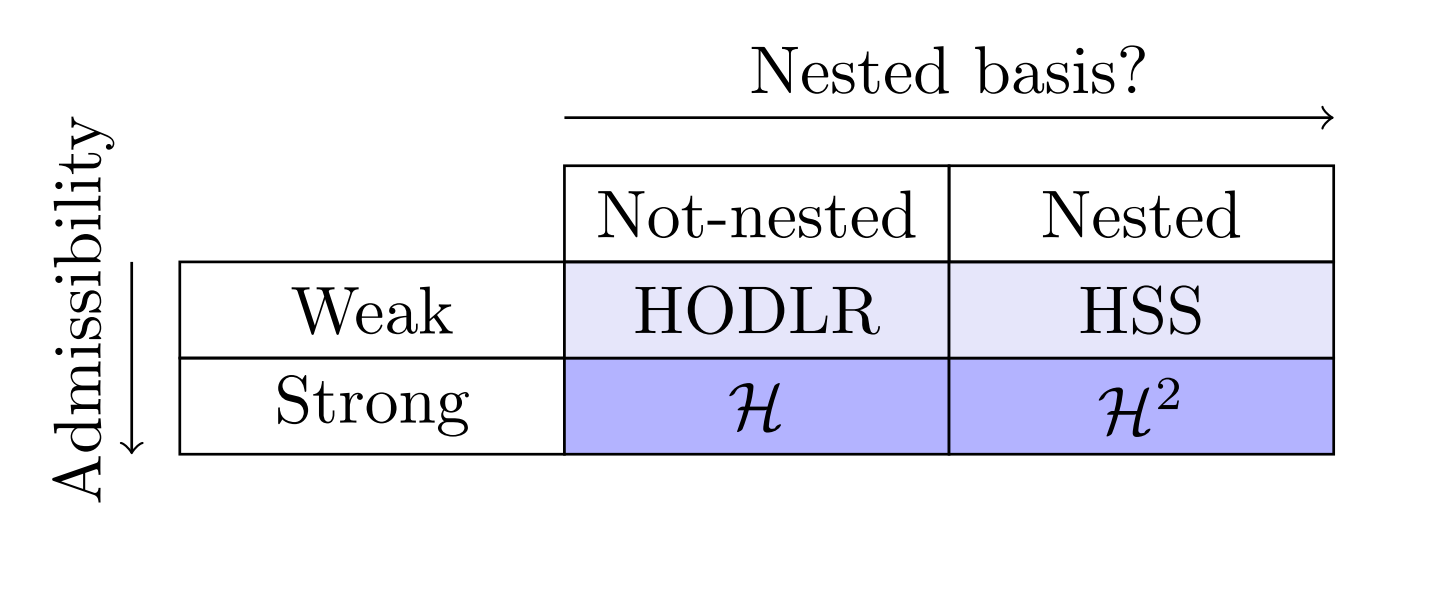
\includegraphics[width=0.6\textwidth]{table.png}
    \caption{How to classify hierarchical matrices.}
    \label{fig:hierarchical_matrices_2}
\end{figure}

\section{Strong Recursive Skeletonization: RS-S}



\section{Proxy Compression}

Proxy compression is necessary in order to achieve the linear complexity bound of the fast-direct solver powered by RS-S. The idea rests on the principle of representing the far-field particles of a given box $B$, which may contain $O(N)$ particles, with a set of `proxy points' contained on a proxy surface that encloses $B$. This surface is often chosen to be a sphere. By choosing $O(1)$ proxy points, without getting into the details yet of how exactly they are sampled, we are able to obtain the linear complexity we desire.

\begin{figure}[!h]
    \centering
    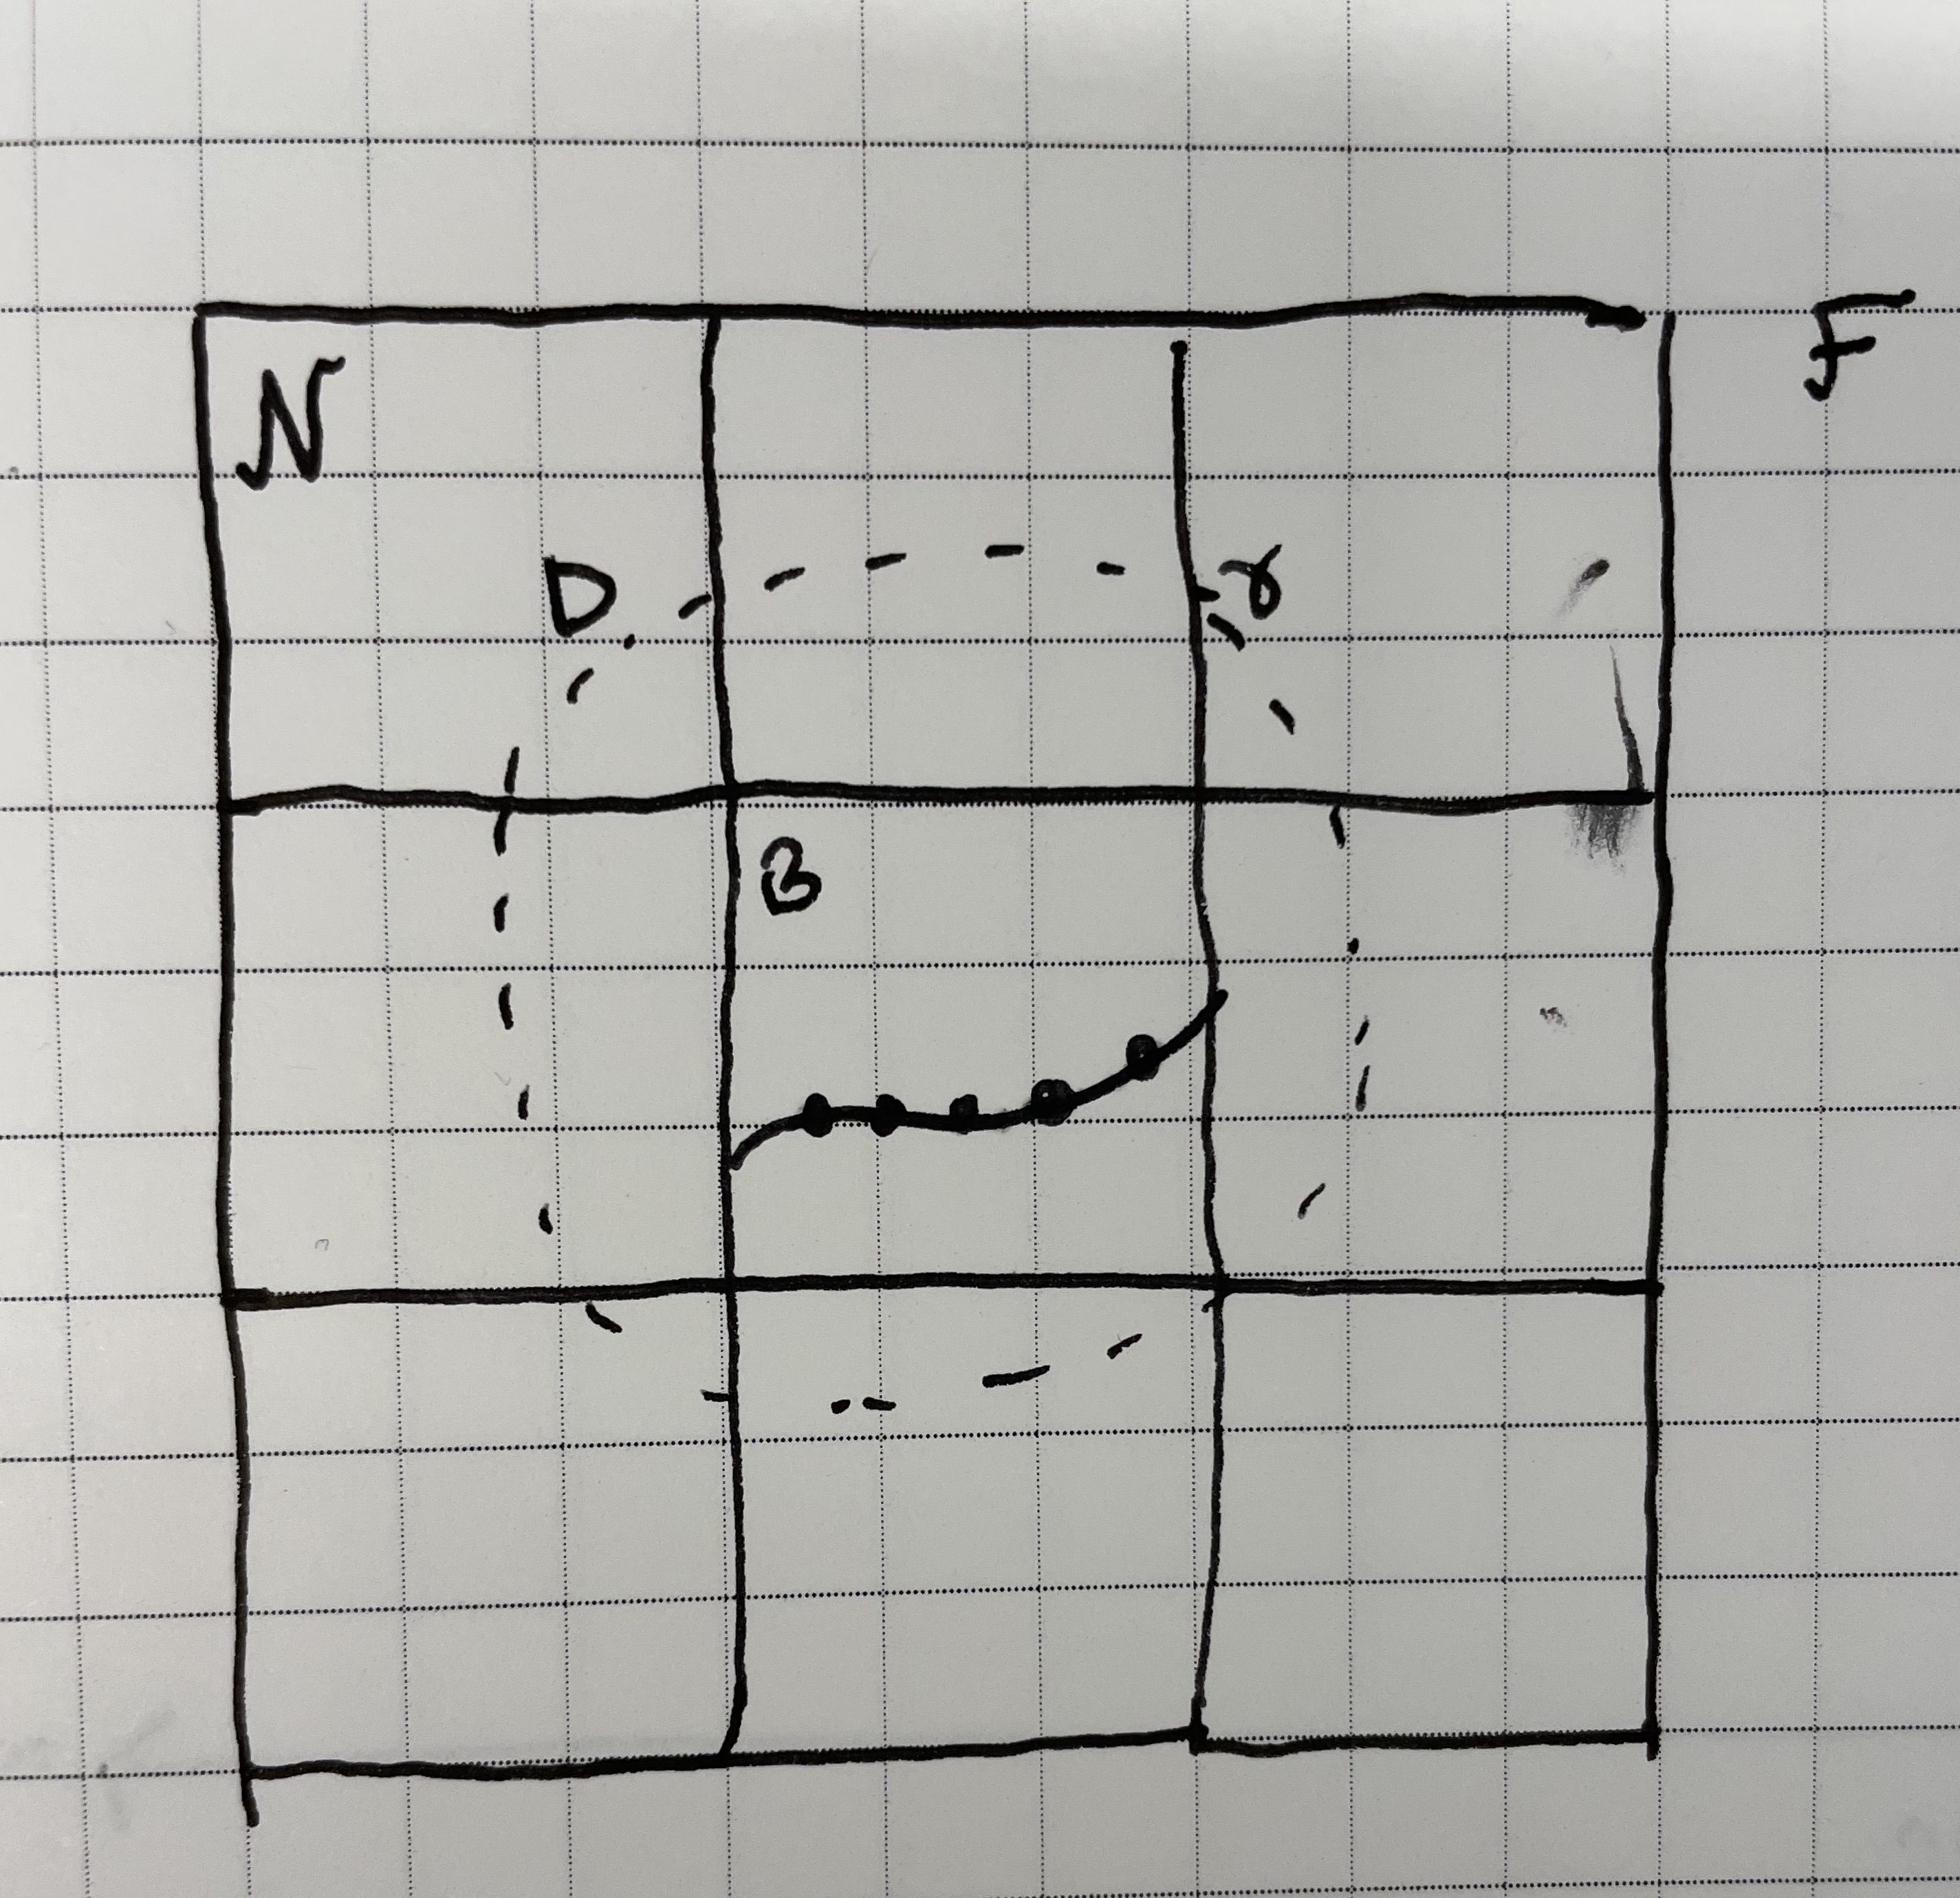
\includegraphics[width=0.6\textwidth]{outgoing_proxy.jpg}
    \caption{Considering the outgoing problem due to charge contained on $\Gamma \cap B$ evaluated in the far-field of $B$.}
    \label{fig:outgoing_proxy}
\end{figure}


For a given box $B$, a proxy surface $D$ and its boundary $\gamma$ are chosen such that $B \subset D$. The far-field points of $B$, $\mathcal{F}$ is partitioned such that $\mathcal{F} = \mathcal{Q} \cup \mathcal{P}$, where $\mathcal{Q}$ contains $O(1)$ points. $\Gamma$ is the boundary of the entire scatterer, and $\tau = \Gamma \cap B$ is the portion of the scatterer boundary contained in $B$. The situation is sketched in figure (\ref{fig:outgoing_proxy}) in 2D.

We can choose to represent our solution due to the charge in $B$ in $\mathcal{F}$ however we wish. However, our choice will lead to different matrices that we must compress.

Generally, we'll end up with a solution matrix of the form $A_{\mathcal{F}B}$ that maps between $B$ and points in its far-field that can be split up as,

\begin{flalign}
    v_{\mathcal{F}} &= A_{\mathcal{F}B} \psi_B \\
    &= B_{\mathcal{F}\gamma} C_{\gamma B} \psi_B
\end{flalign}

the subscripts indicate the domains these operators map between. We desire a split like this, as the far field interaction of $B$ can be compressed into something involving $C_{\gamma B}$.

To see this, consider the fact that $A_{\mathcal{F}B}$ can be written as,

\begin{flalign}
    \label{eq:decomposition}
    A_{\mathcal{F}B} = \begin{bmatrix}
        A_{\mathcal{Q}B}\\ A_{\mathcal{P}B}
        \end{bmatrix} = \begin{bmatrix}
        I & 0\\ 0 & B_{\mathcal{P}\gamma}
        \end{bmatrix} \begin{bmatrix}
        A_{\mathcal{Q}B}\\ C_{\gamma B}
        \end{bmatrix}
\end{flalign}

Our RS-S algorithm relies on a compression of this matrix, however a direct compression of $A_{\mathcal{F} B}$ is too expensive, as there are typically $O(N)$ points in $\mathcal{F}$ for a box $B$, therefore assembly of this matrix for all boxes will result in an algorithm of $O(N^2)$ complexity. However if we can find a decomposition like above, we can apply an interpolative decomposition to the right column in (\ref{eq:decomposition}) which has dimensions $O(1) \times O(n_\gamma)$ by construction where $n_\gamma$ is the number of proxy points. To prove that this allows us to reconstruct the full matrix after compression. Consider an ID that gives us,

\begin{flalign}
    \begin{bmatrix}
        A_{\mathcal{Q}B}\\ C_{\gamma B}
        \end{bmatrix} = \begin{bmatrix}
            A_{\mathcal{Q}S}\\ C_{\gamma S}
        \end{bmatrix} \begin{bmatrix}T_{SR}  & 1 \end{bmatrix}
\end{flalign}

Where $S$ and $R$ are the skeleton and redundant points respectively. Plugging back into our expression (\ref{eq:decomposition}),

\begin{flalign}
    \label{eq:compressed}
    A_{\mathcal{F}B} &=
        \begin{bmatrix}
            I & 0\\ 0 & B_{\mathcal{P}\gamma}
        \end{bmatrix}
        \begin{bmatrix}
             A_{\mathcal{Q}S}\\ C_{\gamma S}
        \end{bmatrix}
        \begin{bmatrix}T_{SR}  & 1 \end{bmatrix} \\
        &=\begin{bmatrix}
            A_{\mathcal{Q}S}\\ B_{\mathcal{P} \gamma}C_{\gamma S}
       \end{bmatrix} \begin{bmatrix}T_{SR}  & 1 \end{bmatrix} \\
       &=  A_{\mathcal{F}S} \begin{bmatrix}T_{SR}  & 1 \end{bmatrix}
\end{flalign}

Therefore, we see that we can get away with a cheap ID to reconstruct the far-field operator, involving the proxy points rather than the full far field of $B$.

\subsection{$\mathcal{T}$}

\subsubsection{Outgoing Skeletonization}

A double-layer potential, due to some unknown density $\psi$, supported on $\tau$,

\begin{flalign}
    v(x) = \int_{\Gamma \cap B} \frac{\partial \Phi(x, y)}{\partial n(y)} \psi(y) ds(y) := \mathcal{D}\psi, \> \> x \in \mathbb{R}^m \setminus \tau
\end{flalign}

solves the Helmholtz equation everywhere it's valid. Here, $\Phi(x, y)$ is the fundamental solution of the Helmholtz equation. However, its normal derivative evaluated at the target points, which we'll need for deriving boundary integral equations for Maxwell problems, does not,

\begin{flalign}
    \frac{\partial v}{\partial n(x)} = \frac{\partial}{\partial n(x)} \int_{\Gamma \cap B} \frac{\partial \Phi(x, y)}{\partial n(y)} \psi(y)ds(y) := \mathcal{T}\psi, \> \> x \in \Gamma \cap \mathcal{F}
\end{flalign}

it's only valid at far-field points, $\Gamma \cap \mathcal{F}$. However, we can separate out the normal part of the derivative,

\begin{flalign}
    \frac{\partial v}{\partial n(x)} = n(x) \cdot \nabla_x \int_{\Gamma \cap B} \frac{\partial \Phi(x, y)}{\partial n(y)} \psi(y)ds(y) := n \cdot w
\end{flalign}

The function

\begin{flalign}
    w(x) = \nabla_x \int_{\Gamma \cap B} \frac{\partial \Phi(x, y)}{\partial n(y)} \psi(y)ds(y) := \nabla_x \mathcal{D}\psi
\end{flalign}

Does satisfy our PDE, everywhere, and we'll exploit this fact in a moment. As an aside, we can see that this is true by considering a double layer potential $v$ that is smooth enough to admit,

\begin{flalign}
    (\Delta + k^2)w =(\Delta + k^2)\nabla_x v =\nabla_x (\Delta + k^2) v = 0
\end{flalign}

where the last equality follows as $v$ satisfies the Helmholtz equation. Therefore $w$ is a solution of the Helmholtz equation. Note that $w$ has three components.

In order to find our $C_{\gamma B}$ with this representation, we need to set up an `associated boundary value problem' for each component of $w$. The choice of boundary value problem we choose is free, as we only rely on the existence of its solution.

Consider an associated boundary value problem for just a single component of $\tilde{w}$ that satisfies,

\begin{flalign}
    &(\Delta + k^2)\tilde{w} = 0, \> \> x \in \mathbb{R}^m \setminus D \\
    &\tilde{w} = w_1(x) \\
    &\text{A radiation condition at } \infty
\end{flalign}

A combined field representation might be nice, as we know it has good properties,

\begin{flalign}
    \tilde{w} = (\mathcal{D} - ik \mathcal{S})_{\mathcal{F}\gamma} \mu
\end{flalign}

where $\mu$ is some unknown density supported on the proxy surface $\gamma$. Forming the boundary integral equation, and plugging back into the representation for $\tilde{w}$,

\begin{flalign}
    \tilde{w} &=  (\mathcal{D} - ik \mathcal{S})_{\mathcal{F} \gamma}(\frac{1}{2}\mathcal{I} + \mathcal{D} - ik \mathcal{S})_{\gamma \gamma}^{-1}w_1 \\
    &= (\mathcal{D} - ik \mathcal{S})_{\mathcal{F} \gamma}(\frac{1}{2}\mathcal{I} + \mathcal{D} - ik \mathcal{S})_{\gamma \gamma}^{-1} \nabla_1 \mathcal{D}_{\gamma B} \psi_\gamma \\
    &\equiv B_{\mathcal{F}\gamma} C_{\gamma B} \psi_\gamma
\end{flalign}

where we identify,

\begin{flalign}
    C_{\gamma B} = \nabla_1 \mathcal{D}_{\gamma B}
\end{flalign}

This is the matrix we will attempt to compress. Similar analysis follows for the other two components of $w(x)$. Meaning that we end up having to compress $[\nabla_1 \mathcal{D}_{\gamma B} , \nabla_2 \mathcal{D}_{\gamma B} , \nabla_3 \mathcal{D}_{\gamma B}]$ for the outgoing problem.

We see that $B_{\mathcal{F} \gamma }$ is never explicitly formed, we just require its existence. When we calculate an approximation of $A_{\mathcal{F}B}$ using (\ref{eq:compressed}), we only need to know the ID of the $C_{\gamma B}$.

\subsubsection{Incoming Skeletonization}

For the incoming skeletonization, were again we're considering the same representation with a hypersingular operator, we observe that we're just looking for,

\begin{flalign}
    \left [\frac{\partial v}{\partial n(x)} \right ]_{\mathcal{F} B}^T
\end{flalign}

with the formation of an associated boundary integral equation taking place in much the same way as for the outgoing problem. However, the double layer operator is self-adjoint, therefore it leads to the same expressions for $C_{\gamma B}$.

\subsection{$\mathcal{K}'$}

\subsubsection{Outgoing Skeletonization}

If we choose to represent our potential with a single-layer potential,

\begin{flalign}
    u(x) = \int_{\Gamma \cap B} \Phi(x, y) \phi(y) ds(y) := \mathcal{S}\phi, \> \> x \in \mathbb{R}^m \setminus D
\end{flalign}

and seek a boundary integral equation in terms of its normal derivative at the targets,

\begin{flalign}
    w(x) = \int_{\Gamma \cap B} \frac{\partial \Phi(x, y)}{\partial n(x)} \phi(y) ds(y) := \mathcal{K}'\phi, \> \> x \in \Gamma \cap \mathcal{F}
\end{flalign}

We observe the same problem as in the $\mathcal{T}$ case, where this expression is not a general solution of our PDE. We can similarly separate out the normal component and write,

\begin{flalign}
    \tilde{w}(x) := \int_{\Gamma \cap B} \nabla_x \Phi(x, y) \phi(y) ds(y), \> \> x \in \mathbb{R}^m \setminus D
\end{flalign}

Using the previous analysis for $\mathcal{T}$, we immediately recognise that the components we must compress are $C_{\gamma B} = \nabla_1 \mathcal{S}_{\gamma B}$, giving us $[\nabla_1 \mathcal{S}_{\gamma B}, \nabla_2 \mathcal{S}_{\gamma B}, \nabla_3 \mathcal{S}_{\gamma B}]$ to compress in total for the outgoing problem.

\subsubsection{Incoming Skeletonization}

Noticing that,

\begin{flalign}
    \left [\frac{\partial u}{\partial n(x)} \right ]_{\mathcal{F} B}^T = \int_{\Gamma \cap B} \frac{\partial \Phi(x, y)}{\partial n(y)} \phi(y) ds(y) = \mathcal{D}_{\gamma B} \phi
\end{flalign}

already satisfies our PDE without any further work, we can save a lot of work, and simply use it as our Dirichlet data in the associated boundary value problem. The matrix to compress being $C_{\gamma B} = \mathcal{D}_{\gamma B}$.

\section{Example Problems}

Let's now apply our fast direct solver framework, with proxy compression to some example problems. We begin with acoustic sound-hard scattering, which is a didactic example.

\subsection{Acoustic Sound Hard Scattering}

Consider a scattered field $u^s$, that bounces off an object $\Omega$ and satisfies the Helmholtz equation in the exterior,

\begin{flalign}
    (\Delta + k^2)u^s = 0, \> \> \> \text{in  } \mathbb{R}^3 \setminus \Omega
\end{flalign}

The `sound hard' boundary condition on the surfae $\Gamma$ is
\begin{flalign}
    \frac{\partial u^s}{\partial n} = \frac{\partial u^{i}}{\partial n}, \> \> \> \text{in  } \Gamma
\end{flalign}

where $u^i$ is the incident wave. Using the analysis in \cite{Bruno2012}, we write down a `regularised' representation formula for our solution. This regularisation can be shown to have better spectral properties.

\begin{flalign}
    u^s =(\mathcal{K}_k \circ \mathcal{S}_K - i\eta \mathcal{S}_k)
\end{flalign}

where $k$ and $K$ are complex wave numbers, that may not be the same. We can take the trace of this representation, and its normal derivative at the targets, and find a boundary integral equation for the exterior problem,

\begin{flalign}
    (\frac{i \eta}{2} \mathcal{I}- i \eta \mathcal{K}'_k + \mathcal{T}_k \circ \mathcal{S}_K )\mu = g
\end{flalign}

using the Calder\'{o}n identity,

\begin{flalign}
    \mathcal{T}_k\circ \mathcal{S}_k = -\frac{1}{4}\mathcal{I} + \mathcal({K}_k')^2
\end{flalign}

which is true for any $k$, we arrive at a boundary integral equation,

\begin{flalign}
    \left ( i \eta(\frac{1}{2}\mathcal{I}  - \mathcal{K}'_k) - \frac{1}{4}I+ \mathcal({K}_k')^2 \right ) \mu = g
\end{flalign}

by defining $\theta := \mathcal{K}'_k \mu$, we can write the boundary integral equation as a system,

\begin{flalign}
\begin{pmatrix}
(\frac{i\eta}{2} - \frac{1}{4})\mathcal{I} - i \eta \mathcal{K}'_k & \mathcal{K}'_k  \\
 \mathcal{K}'_k & - \mathcal{I}
\end{pmatrix}
\begin{pmatrix} \mu \\ \theta \end{pmatrix} = \begin{pmatrix}
    g \\ 0
\end{pmatrix}
\end{flalign}

We can then place this system into our fast direct solver framework. Despite not knowing how to compress the system matrix altogether, we do know how to compress each block, as they each correspond to displacements of $\mathcal{K}'_k$.

Consider writing out our block matrix as,


\begin{flalign}
    \begin{pmatrix}
        A & B \\ C & D
    \end{pmatrix}
    \begin{pmatrix}
        \mu\\\theta
    \end{pmatrix}
   = \begin{pmatrix}
        g\\ 0
    \end{pmatrix}
\end{flalign}

and re-writing as,

\begin{flalign}
    \begin{pmatrix}
        \begin{pmatrix}
            A_{11} & B_{11} \\ C_{11} & D_{11}
        \end{pmatrix} & . & .\\
        . & . & \\
        . & &     \begin{pmatrix}
            A_{NN} & B_{NN} \\ C_{NN} & D_{NN}
        \end{pmatrix}
    \end{pmatrix}
    \begin{pmatrix}
        \mu_1 \\ \theta_1 \\ . \\ . \\ \mu_n \\ \theta_n
    \end{pmatrix} =
    \begin{pmatrix}
        g_1 \\ 0 \\ . \\ . \\ g_N \\ 0
    \end{pmatrix}
\end{flalign}

This system matrix remains numerically low-rank, and therefore can fit into our FDS framework. Indeed, we now have to compress a system of matrix operators in order to capture its row space via the proxy trick,

\begin{flalign}
    f
\end{flalign}

\subsection{Acoustic Transmission}

\subsection{Maxwell Scattering}

\end{document}


